\documentclass[addpoints]{exam}

\printanswers
\CorrectChoiceEmphasis{\color{red}\bfseries}
\usepackage{amssymb, amsmath, amsfonts}
\usepackage{geometry}
\usepackage{graphicx}
\usepackage{tikz}
\usetikzlibrary{calc}
\usepackage{pgfplots}
\usepackage{multirow,array} % for payoff matrix formatting
\usepackage[colorlinks,pdfusetitle,urlcolor=blue,citecolor=blue,linkcolor=blue]{hyperref}

\definecolor{crimson}{RGB}{ 170, 4, 36 }
\definecolor{darkblue}{RGB}{ 4, 47, 170 }
\definecolor{brown}{RGB}{ 111, 71, 2 }
\definecolor{periwinkle}{RGB}{ 90, 177, 204 }
\definecolor{ducksgreen}{HTML}{007030}

\geometry{left=1.0in,right=1.0in,top=1.0in,bottom=1.0in}
\pagestyle{headandfoot}
\lhead{EC327 Game Theory}
\chead{Homework 4}
\rhead{Fall 2025}
\runningheadrule

\title{
    \textbf{Econ 327: Game Theory} \\ 
    Homework $\#4$
    }
\author{University of Oregon}
\date{Due: Oct. 24$^{th}$}

% exam-type question formatting
\renewcommand{\thequestion}{\textbf{Q\arabic{question}}}
\bracketedpoints

\begin{document}

\maketitle

\begin{center}
  \gradetable[h][questions]
\end{center}

\vspace{0.5in}

\begin{center}
  \textbf{For homework assignments:}
\end{center}

\begin{itemize}

%  \item DO NOT write your name:
%  this assignment will be graded anonymously. 
%  If you want to, you can include your student ID instead.

  \item Complete \textit{all} questions and parts.

  % I will select one question at random to be graded
  % according to the rubric on Canvas.

  \item You will be graded on not only the content of your work
    but on how clearly you present your ideas.
    Make sure that your handwriting is legible.
    Please use extra pages if you run out of space 
    but make sure that all parts of a question 
    are in the correct order when you submit.

  \item You may choose to work with others,
  but everyone must submit to Canvas individually.

  Please include the names of everyone who you worked with 
  below your own name.
 
\end{itemize}

\vspace{1.0in}

\makebox[.6\textwidth]{Name\enspace\hrulefill}

\vspace{0.5in}

% \begin{center}
%   \fbox{\fbox{\parbox{5.5in}{\centering
%     Answer the questions in the spaces provided on the
%     question sheets. If you run out of room for an answer,
%     continue on the back of the page or another sheet of paper.}}}
% \end{center}

\begin{questions}

\newpage

\question
Recall the gnu and croc river crossing game from Homework 2, Question 3.

Now, consider what happens if the gnu have bad eyesight and can't see where the crocs are choosing to lie in wait.

\begin{parts}
  
\part[4]
Draw out the new extensive form game.

\begin{solution}
  Either of the following extensive forms is acceptable:

  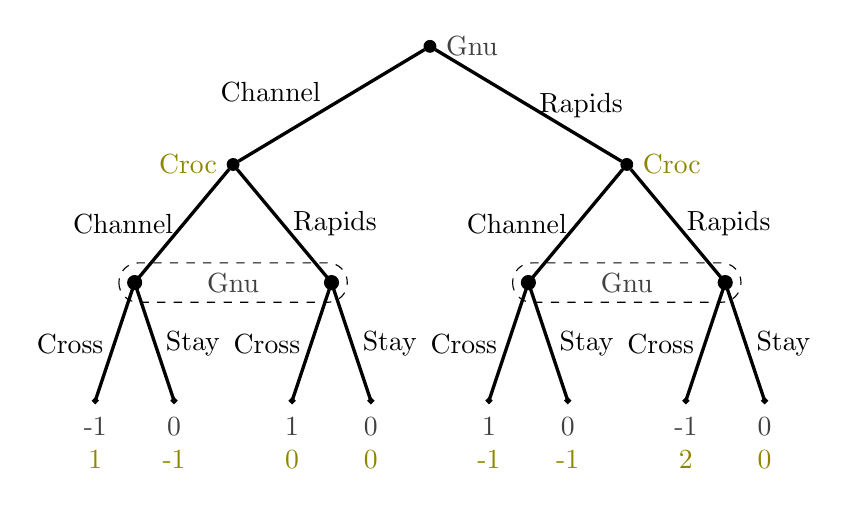
\begin{tikzpicture}[edge from parent/.style={draw, very thick}]
    \tikzstyle{solid node}=[circle,draw,inner sep=1.5,fill=black]
    \tikzstyle{hollow node}=[circle,draw,inner sep=.25]
    \tikzstyle{level 1}=[level distance=15mm,sibling distance=5cm]
    \tikzstyle{level 2}=[level distance=15mm,sibling distance=2.5cm]
    \tikzstyle{level 3}=[level distance=15mm,sibling distance=1cm]
    \tikzstyle{pruned edge from parent}=[draw, very thick, darkgray, dashed, -]
    
    \node(0)[solid node,label=right:{\color{darkgray} Gnu}]{}
        child{node[solid node,label=left:{\color{olive} Croc }]{}
            child{node(1)[solid node]{}
                child{node[hollow node,label=below:{
                    \begin{tabular}{c}
                         {\color{darkgray} -1}  \\
                         {\color{olive} 1} 
                    \end{tabular}
                }]{} edge from parent node[left]{Cross}}
                child{node[hollow node,label=below:{
                    \begin{tabular}{c}
                         {\color{darkgray} 0}  \\
                         {\color{olive} -1} 
                    \end{tabular}
                }]{} edge from parent node[right]{Stay}}
            edge from parent node[left]{Channel}}
            child{node(2)[solid node]{}
                child{node[hollow node,label=below:{
                    \begin{tabular}{c}
                         {\color{darkgray} 1}  \\
                         {\color{olive} 0} 
                    \end{tabular}
                }]{} edge from parent node[left]{Cross}}
                child{node[hollow node,label=below:{
                    \begin{tabular}{c}
                         {\color{darkgray} 0}  \\
                         {\color{olive} 0} 
                    \end{tabular}
                }]{} edge from parent node[right]{Stay}}
            edge from parent node[right]{Rapids}}
            edge from parent node[left,xshift=0,yshift=5]{Channel}
        }
        child{node[solid node,label=right:{\color{olive} Croc }]{}
            child{node(3)[solid node]{}
                child{node[hollow node,label=below:{
                    \begin{tabular}{c}
                         {\color{darkgray} 1}  \\
                         {\color{olive} -1} 
                    \end{tabular}
                }]{} edge from parent node[left]{Cross}}
                child{node[hollow node,label=below:{
                    \begin{tabular}{c}
                         {\color{darkgray} 0}  \\
                         {\color{olive} -1} 
                    \end{tabular}
                }]{} edge from parent node[right]{Stay}}
            edge from parent node[left]{Channel}}
            child{node(4)[solid node]{}
                child{node[hollow node,label=below:{
                    \begin{tabular}{c}
                         {\color{darkgray} -1}  \\
                         {\color{olive} 2} 
                    \end{tabular}
                }]{} edge from parent node[left]{Cross}}
                child{node[hollow node,label=below:{
                    \begin{tabular}{c}
                         {\color{darkgray} 0}  \\
                         {\color{olive} 0} 
                    \end{tabular}
                }]{} edge from parent node[right]{Stay}}
            edge from parent node[right]{Rapids}}
            edge from parent node[right]{Rapids}
        }
        ;
% information set
\draw[dashed,rounded corners=7]($(1)+(-.2,.25)$)rectangle($(2)+(.2,-.25)$);
\draw[dashed,rounded corners=7]($(3)+(-.2,.25)$)rectangle($(4)+(.2,-.25)$);
% specify movers
\node at ($.5*(1)+.5*(2)$) {\color{darkgray} Gnu};
\node at ($.5*(3)+.5*(4)$) {\color{darkgray} Gnu};
\end{tikzpicture}


  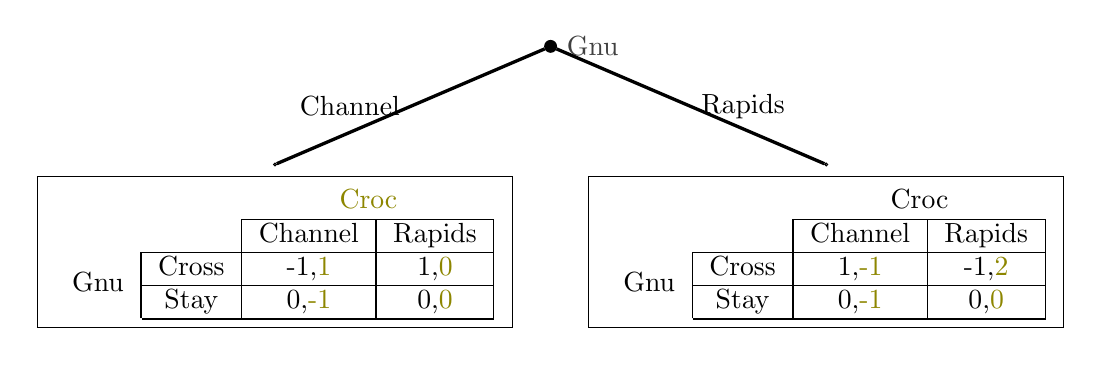
\begin{tikzpicture}[edge from parent/.style={draw, very thick}]
    \tikzstyle{solid node}=[circle,draw,inner sep=1.5,fill=black]
    \tikzstyle{hollow node}=[circle,draw,inner sep=.25]
    \tikzstyle{level 1}=[level distance=15mm,sibling distance=7cm]
    \tikzstyle{pruned edge from parent}=[draw, very thick, darkgray, dashed, -]
    
    \node(0)[solid node,label=right:{\color{darkgray} Gnu}]{}
      child{node[hollow node,label=below:{
        \fbox{
        \begin{tabular}{*{4}{c|}}
           \multicolumn{2}{c}{} & \multicolumn{2}{c}{\color{olive} Croc} \\\cline{3-4}
           \multicolumn{1}{c}{} &       & Channel & Rapids \\\cline{2-4}
           \multirow{2}*{Gnu}   & Cross & -1,{\color{olive}1}  & 1,{\color{olive}0}   \\\cline{2-4}
                                & Stay  & 0,{\color{olive}-1}  & 0,{\color{olive}0}   \\\cline{2-4}
        \end{tabular}
        }
      }]{}
          edge from parent node[left]{Channel}
      }
      child{node[hollow node,label=below:{
        \fbox{
        \begin{tabular}{*{4}{c|}}
           \multicolumn{2}{c}{} & \multicolumn{2}{c}{Croc} \\\cline{3-4}
           \multicolumn{1}{c}{} &       & Channel & Rapids \\\cline{2-4}
           \multirow{2}*{Gnu}   & Cross & 1,{\color{olive}-1}  & -1,{\color{olive}2}   \\\cline{2-4}
                                & Stay  & 0,{\color{olive}-1}  &  0,{\color{olive}0}   \\\cline{2-4}
        \end{tabular}
        }
      }]{}
          edge from parent node[right]{Rapids}
      }
      ;
\end{tikzpicture}

\end{solution}

\part[4]
First, solve for all Nash equilibria in every proper \textit{subgame} of the extensive form game tree.

\begin{solution}

  In the subgame following the gnu choosing Channel,
  the only Nash is in mixed strategies which is when the gnu \textbf{Cross 50\% of the time} (and stay 50\% of the time) and the crocs wait in the \textbf{Channel 50\% of the time} (and wait in the rapids 50\% of the time).

  In the subgame following the gnu choosing Rapids,
  the only Nash is in pure strategies where the gnu \textbf{Stay} and the crocs wait in the \textbf{Rapids}.
\end{solution}
  \part[4]
  How does your prediction change from homework 2?
  Would you still expect to always see the gnu safely crossing at the channel?

  \begin{solution}
    If the Gnu can't see the Crocs, they can't use a strategy where they only selectively cross the Channel if the Crocs are there.
    If they choose to Cross the Channel in this case, then the Crocs will decide it's worth it to go to the Channel.
    So the equilibrium from earlier doesn't apply because the information sets of the extensive form game have changed.
  \end{solution}

\end{parts}

\newpage

\question
Consider the extensive form game treee below.

\begin{center}
  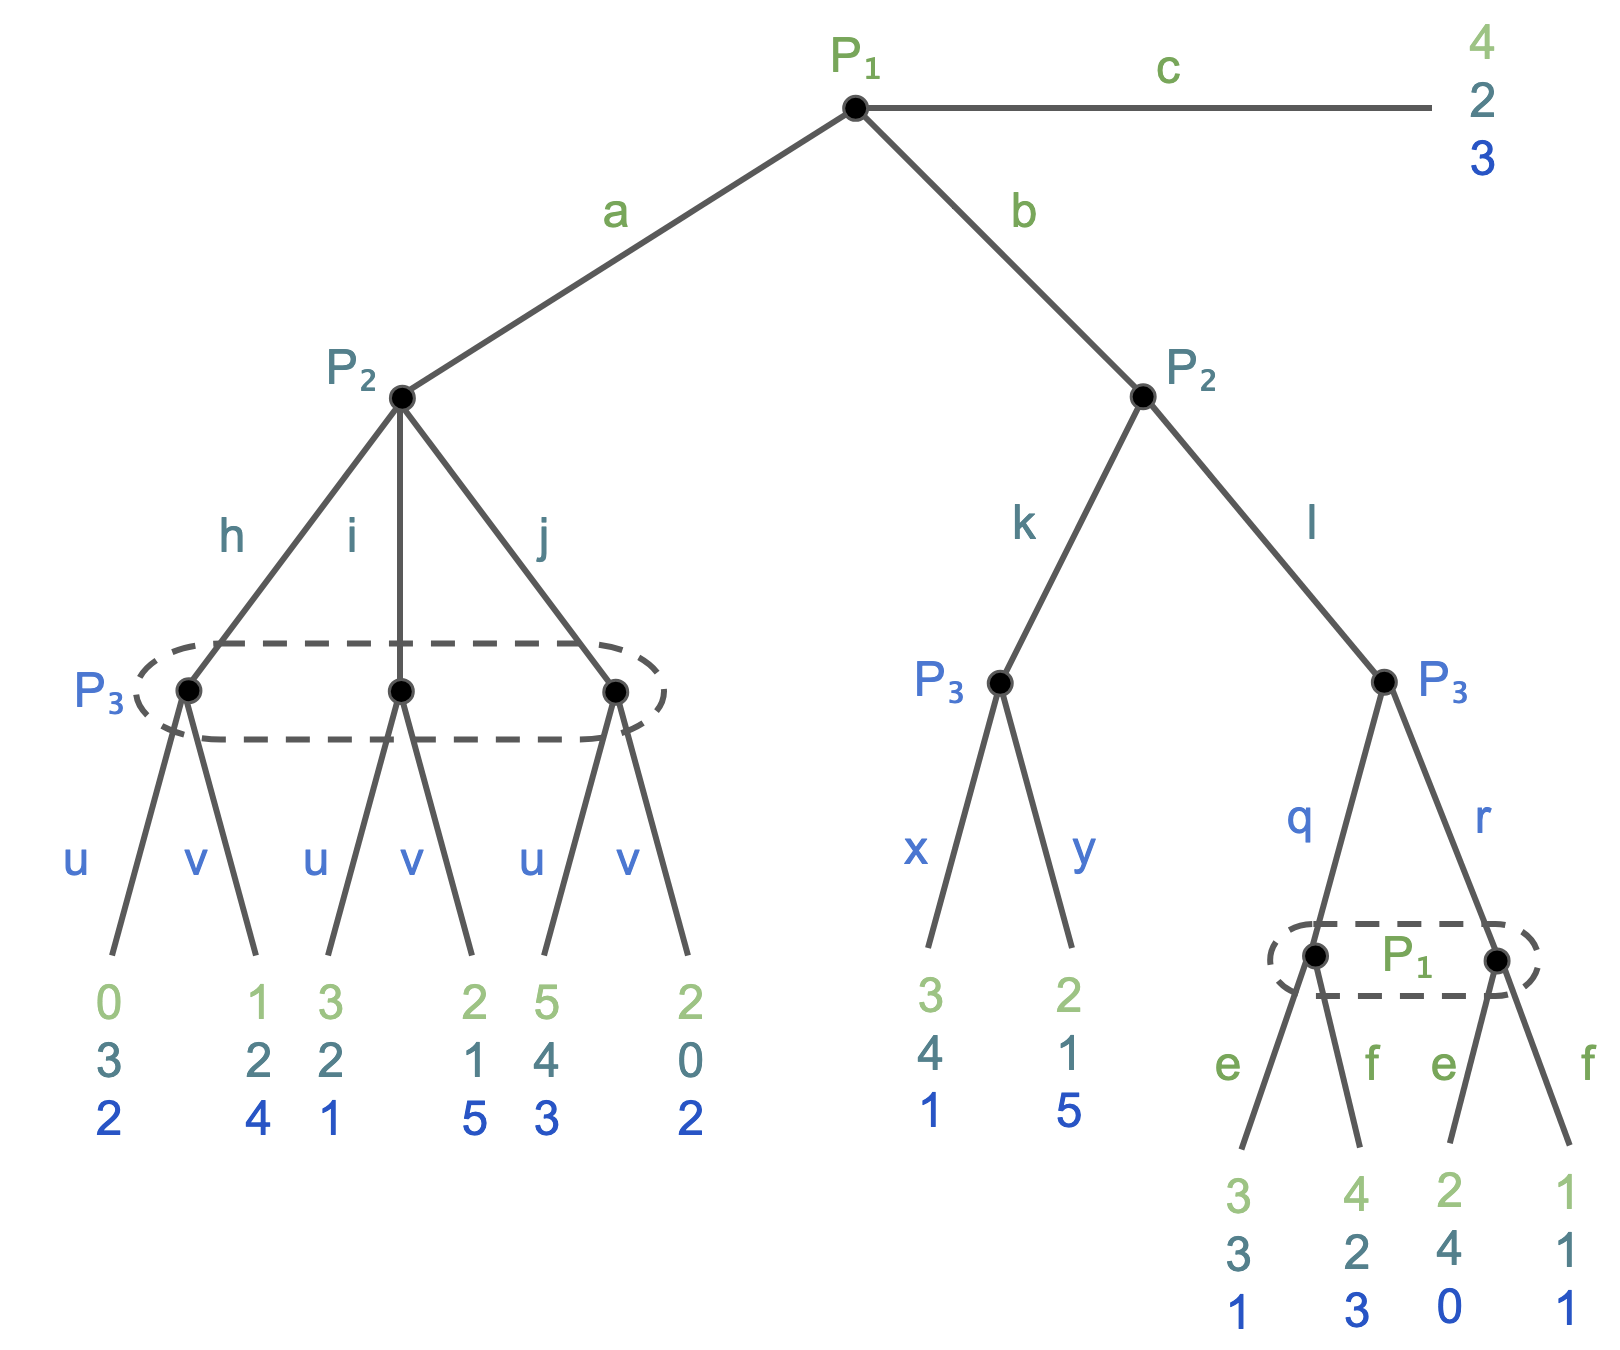
\includegraphics[width = .8\textwidth]{figures/bigtree.png}
\end{center}

\begin{parts}
  
  \part[2] 
  What should a complete strategy profile look like?

  How many elements will each player have in their \textit{complete} strategy?

  \part[4] Find all subgame perfect Nash equilibria in pure strategies.

  \part[4] Can you find a Nash equilibrium that is not subgame perfect?
  Carefully explain.

\end{parts}

\newpage

\question
A game theorist is walking down the street in his neighborhood and finds \$20.
Just as he picks it up, two neighborhood kids, 
Jane and Tim,
run up to him, asking if they can have it.
Because game theorists are generous by nature, 
he says he's willing to let them have the \$20,
but only according to the following procedure:
Jane and Tim are each to submit a written request 
as to their share of the \$20. 
Let $t$ denote the amount that Tim requests for himself
and $j$ be the amount that Jane requests for herself.
Tim and Jane must choose $j$ and $t$ from the interval
$[0,20]$.
If $j + t \leq 20$, then the two receive what they requested,
and the remainder, $20 - j - t$, is split equally between them.
If, however, $j + t > 20$, then they get nothing, and the game theorist keeps the \$20.
Tim and Jane are the players in this game.
Assume that each of them has a payoff equal to the amount of money that he or she receives. 
\footnote{Harrington \textit{Games, Strategies, and Decision Making}}

\begin{parts}
  \part[4]
  Describe Tim's and Jane's best response rules.
  \begin{solution}

    Tim's best response rule:
    $$ 
    BR_t(j) = \begin{cases}
      20 - j & \text{ if } j < 20 \\
      [0,20] & \text{ if } j = 20
      \end{cases}
    $$
    Jane's best response rule:
    $$ 
    BR_j(t) = \begin{cases}
      20 - t & \text{ if } t < 20 \\
      [0,20] & \text{ if } t = 20
      \end{cases}
    $$
  \end{solution}

  \part[4]
  Find all Nash equilibria. Be careful about corner solutions.
  \begin{solution}
    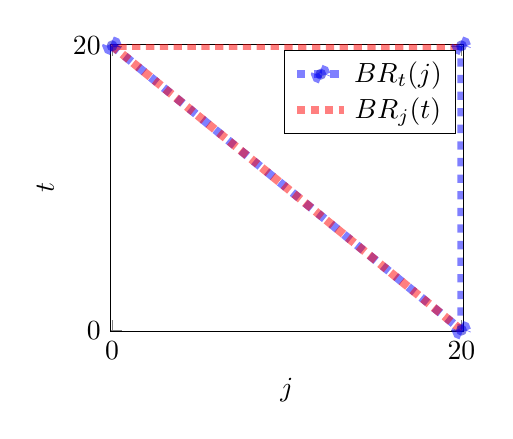
\begin{tikzpicture}
      \begin{axis}[
        width=.5\textwidth,
        xlabel={$j$},
        ylabel={$t$},
        xmin=-0.1, xmax=20.1,
        ymin=-0.1, ymax=20.1,
        xtick={0,20},
        ytick={0,20},
        ]
        \addplot+ [
        dashed,
        line width=3pt,
        color=blue,
        opacity=0.5
        ] 
        coordinates
        {
        (0, 20)
        (20, 0)
        (20, 20)
        };
        \addlegendentry{\(BR_t(j)\)}
        \addplot [
        dotted,
        line width=3pt,
        color=red,
        opacity=0.5
        ] 
        coordinates
        {
          (20,0)
          (0, 20)
          (20,20)
        };
        \addlegendentry{\(BR_j(t)\)}
      \end{axis}
    \end{tikzpicture}
  
    The NE are any points on the graph where the $BR_j(t) = t$ and $BR_t(j) = t$.
    This includes the diagonal line which is the set of all pairs,
    $j$ and $t$ such that $j + t = 20$ where $j,t<20$.
    When $j=20$, there is one NE when $t=0$ and another when $t=20$.
    When $t=20$, there is one NE when $j=0$ (and $j=20$ is still NE).
  
  \end{solution}
\end{parts}

\newpage

\question \textbf{[n-person game theory]}

Suppose there are two types of music fans:
\textit{normies} only like a band if a majority of other people like them too;
\textit{hipsters} only like a band if a minority of other people like them.

Suppose that the payoff to \textit{normies} from liking \textit{Wolf Alice} is $100 + 2m$, where $m$ is the number of people who like them.
The payoff to a \textit{hipster} from liking \textit{Wolf Alice} is $500 - 5m$.
Anyone can choose to like \textit{The National} which has a payoff of 100.

Assume there arre 100 people, 75 are \textit{normies}, and 25 are \textit{hipsters}.
\footnote{Adapted from Cliff Bekar, Lewis \& Clark College}

\begin{parts}
  \part[4]
  Is it a Nash equilibrium for only the \textit{hipsters} to like \textit{Wolf Alice}?
  \begin{solution}

    $u(Wolf~Alice)_{hipsters} =  375 > 100 = u(National)$, so \textit{hipsters} are willing to like $WA$.

    But \textit{normies} also like $WA$ better because
    $u(Wolf~Alice)_{normies} = 150 > 100$.

    So this is not a Nash.
  \end{solution}

  \part[4]
  Is it a Nash equilibrium for only the \textit{normies} to like \textit{Wolf Alice}?
  \begin{solution}
    $u(Wolf~Alice)_{hipsters} =  125 > 100 = u(National)$, so \textit{hipsters} would also like \textit{Wolf Alice}.
    So this is not a Nash.
  \end{solution}

  \part[4]
  Is there a Nash equilibrium where \textit{Wolf Alice} has fans of both types?
  \begin{solution}
    For \textit{hipsters} to be indifferent between $WA$ and $N$, 
    \begin{align*}
      u(WA)_h & = u(N)_h \\
      500 - 5m & = 100 \\ 
      m & = 80
    \end{align*}
    So all \textit{normies} and 5 \textit{hipsters} liking \textit{Wolf Alice} is a Nash equilibrium.
  \end{solution}
\end{parts}
\end{questions}
\end{document}
